\subsection{SD-Card Reader Module (SD) }

The SD-Card Reader Module (SD) allows to write debug data to a standard SD-card. All the information listed in
\ref{sec:DP} is made persistent for further analysis.
Doing so via GSM transmission would be too costly both in terms of energy consumption and in service usage fees.

\subsubsection{Requirements}

SD must offer a SPI or UART interface because the I2C bus is already used for master-slave communication.
The operating voltage must be either \SI{3.3}{\volt} or \SI{5}{\volt}.

\subsubsection{Implementation}

We use an Arduino-compatible MicroSD Card shield available on various online retailers.

\begin{figure}[h]
    \centering
    \includegraphics[width=1.0\textwidth]{SL/SD/SD}
    \caption{SD - schematic}

\end{figure}


\begin{table}[H]
    \centering
    \begin{threeparttable}[b]
        \begin{tabularx}{\linewidth}{ >
                    {\hsize=.25\hsize}X >
                    {\hsize=0.5\hsize}X >
                    {\hsize=.25\hsize}X  >
                    {\hsize=.5\hsize}X >
                    {\hsize=.25\hsize}X  >
                    {\hsize=3\hsize}X
            }
                  & \multicolumn{4}{c}{Pin mapping} &                                                 \\
            \cmidrule(lr){3-6}
            Id    & Net                             & Nb. & Name         & Type            & Function \\
            \midrule
            $U_1$ & .SCK                            & 4   & \texttt{D5}  & \rightharpoonup &          \\
            $U_1$ & .MISO                           & 5   & \texttt{D6}  & \rightharpoonup &          \\
            $U_1$ & .MOSI                           & 6   & \texttt{D7}  & \leftharpoonup  &          \\
            $U_1$ & .CS                             & 7   & \texttt{D8}  & \leftharpoonup  &          \\
            $U_1$ & .3V3                            & 8   & \texttt{D8}  & \leftarrow      &          \\
            $U_1$ & \Gnd                            & 10  & \texttt{GND} & \Gnd            &          \\
        \end{tabularx}
    \end{threeparttable}
    \caption{SD - pin mapping}
\end{table}